\documentclass[sigconf]{acmart}

\settopmatter{printacmref=false} % Removes citation information below abstract
\renewcommand\footnotetextcopyrightpermission[1]{} % removes footnote with conference information in first column
\pagestyle{plain} % removes running headers

\usepackage{graphicx}

\usepackage{balance}  % for  \balance command ON LAST PAGE  (only there!)
\usepackage{booktabs}
\usepackage{algorithm}
\usepackage{algorithmic}
\usepackage{ulem}
\usepackage{color}
\usepackage{epstopdf}

\setlength{\textfloatsep}{2pt}
\setlength{\dbltextfloatsep}{2pt}


\begin{document}
%\small
\title{WebPut: A Web-Aided Data Imputation System for the General Type of Missing String Attribute Values}

%\author{Shuangli Shan}
%\affiliation{%
%  \institution{The School of Computer Science and Technology, Soochow University, China}
%}
%\email{sldan@stu.suda.edu.cn}
%
%\author{Zhixu Li}
%\authornote{Corresponding author}
%\affiliation{%
%  \institution{The School of Computer Science and Technology, Soochow University, China}
%}
%\email{zhixuli@suda.edu.cn}
%
%\author{Yang Li}
%\affiliation{%
%  \institution{The School of Computer Science and Technology, Soochow University, China}
%}
%\email{yang.li6@hotmail.com}
%
%\author{Qiang Yang}
%\affiliation{%
%  \institution{The School of Computer Science and Technology, Soochow University, China}
%}
%\email{qiangyanghm@hotmail.com}
%
%\author{Jia Zhu}
%\affiliation{%
%  \institution{South China Normal University, China}
%}
%\email{jzhu@m.scnu.edu.cn}
%
%\author{Mohamed Sharaf}
%\affiliation{%
%  \institution{The University of Queensland, Brisbane, Australia}
%}
%\email{fmsharaf@itee.uq.edu.au}
%
%\author{Xiaofang Zhou}
%\affiliation{%
%  \institution{The University of Queensland, Brisbane, Australia}
%}
%\email{zxf@itee.uq.edu.au}

% The default list of authors is too long for headers.
%\renewcommand{\shortauthors}{B. Trovato et al.}


\begin{abstract}
%Data imputation aims at filling in missing attribute values in databases. While traditional imputation systems rely on constraints such as FD/CFDs or trained prediction models, recent work turn to crowdsourcing for help. However, traditional model frequently failed to get the right answers for the lack of enough knowledge, while the crowd-based methods struggle in reducing the cost of human interventions.
In this demonstration, we present an end-to-end web-aided data imputation prototype system named WebPut. WebPut consults the Web for imputing the missing values in a local database when the traditional inferring-based imputation method has difficulties in getting the right answers.
%
Specifically, WebPut investigates the interaction between the local inferring-based imputation methods and the web-based retrieving methods and shows that retrieving a small number of selected missing values can greatly improve the imputation recall of the inferring-based methods.
%
Besides, WebPut also incorporates a crowd intervention component that can get advice from humans in case that the web-based imputation methods may have difficulties in making the right decisions.
%
We demonstrate, step by step, how WebPut fills an incomplete table with each of its components. %Meanwhile, for the comparison purpose, we will also show the imputation results of some other methods.
\end{abstract}

%
% The code below should be generated by the tool at
% http://dl.acm.org/ccs.cfm
% Please copy and paste the code instead of the example below.
%

\maketitle

\section{Introduction}

Having missing values is a common problem for databases, and the process of filling in the missing attribute values is well known as data imputation~\cite{li2012webput, wang2002empirical}. So far, various imputation methods have been developed for missing quantitive data (either continuous or discrete data), while only limited attention has been paid to non-quantitive data (pure string data with a large scope of values)~\cite{li2015trip}. However, pure string data takes up a large part of the missing data in many databases, and it can be seen as a general type of data since all kinds of data can be taken as a special type of string data.


Existing imputation methods to the general type of non-quantitive string data mainly rely on some local data constraints (such as FD/CFDs)~\cite{wu2004using, shen2007combined, bohannon2007conditional} or some prediction models~\cite{wang2002empirical, zhang2008parimputation} to infer substitutes or estimations for the missing values. However, the inferring-based methods always fail to get the right missing value for the lack of enough knowledge, especially when the missing value is unique in the data set. Considering the drawbacks of the previous methods, some systems turn to involve crowdsourcing for help, such as outsourcing the task to a crowdsourcing platform to obtain answers from crowd workers~\cite{ye2014capture, franklin2011crowddb}.
%
Crowd-based imputation methods have shown effectiveness on improving imputation precision and recall. A big problem of this kind of methods is to reduce costs the of human interventions which are always expensive. However, it is hard to control the balance between crowdsourcing qualities and costs. Also, human interventions from experts may not always be available, which further reduces the applicability of systems.


Why not use a much cheaper and within reach knowledge depository, i.e., the Web, in data imputation? Compared with crowdsourcing, the Web has at least four advantages: 1) It is almost free. Generally, there is no need to pay for getting information from the surface Web. 2) Consulting the Web through web search engines has no restrictions on time and locations since the Web does not sleep and can be accessed everywhere. 3) Consulting the Web can be very fast especially when it is performed in parallel. 4) As the world's largest repository of human's knowledge, the Web naturally contains enough raw data and knowledge, either structured (such as Wikipedia) or unstructured, supporting the imputation for data in databases of different domains.


These advantages motivate us to develop a Web-Aided Data Imputation (or {\bf WebPut} for short) system, which implements a web-based data imputation module, and employs an interactive way to integrate the web-based imputation with existing inferring-based data imputation methods. Our goal is to minimize the usage of the Web on the condition of satisfying the high quality of data imputation. Besides, a crowdsourcing component is incorporated to get answers from human to help control the quality of imputation results from the Web in a cost-efficient way.
%
To make WebPut a general imputation tool for various types of missing textual values, the current system takes every textual value of a particular type (like numeric, email address, currency) as a kind of string, based on which we design all our imputation techniques on the string data only. As a future work, we will integrate the imputation techniques that are specially designed for some particular data type into the system.


%WebPut utilizes existing attribute values in conjunction with data consistency principle to provide estimations for the missing attribute values, or automatically generates and selects qualified search queries to retrieve the value from the web.
%

\begin{figure}
  % Requires \usepackage{graphicx}
  \centerline{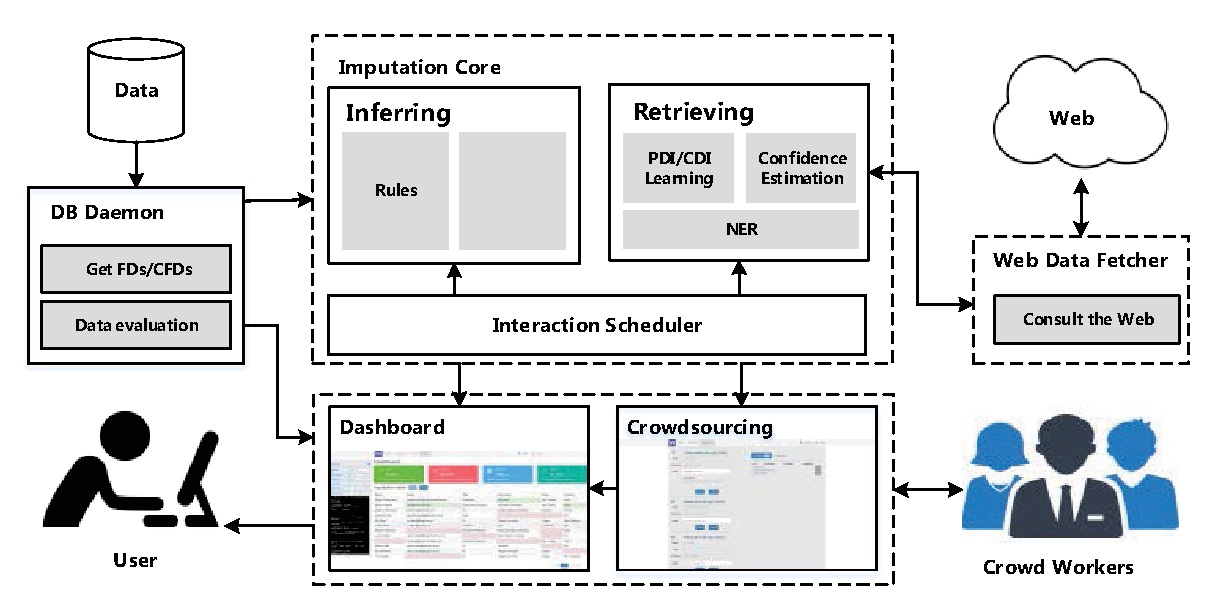
\includegraphics[width=6cm]{images/Architecture.eps}}
  \caption {\small  The System Architecture of WebPut}
  \label{fig:architecture}
\end{figure}

%In the rest of the paper, we first describe the architecture of WebPut in Section 2, and then provide a glimpse of the techniques underlying our work in Section 3. Finally, we discuss our demonstration plan in Section 4.

\vspace{-10pt}
\section{SYSTEM  OVERVIEW}
Fig.~\ref{fig:architecture} shows the building blocks of WebPut. Basically, there are  five main components: the DB Daemon, the Imputation Core, the Web Data Fetcher, the Interaction Scheduler, and the Crowdsourcing Interface. We introduce the design of these components respectively as follows.

\noindent{\bf 1) DB Daemon:} This module is responsible for importing data from databases and collecting quality rules such as FD/CFDs and user-defined rules. In addition, the DB daemon verifies the completeness of all tuples and identifies the missing values for imputation.


\noindent{\bf 2) Imputation Core:} The imputation approaches we adopt in WebPut include both traditional inferring-based imputation method and retrieving-based imputation method.

\noindent\underline{\it (1) Inferring-based Imputation:}
The Inferring-based imputation APPROACH we adopt in WebPut relies on data constraints, such as FD/CFDs, to infer the missing values from the complete part of the dataset~\cite{kolahi2009approximating, fan2008conditional}.


\noindent\underline{\it (2) Retrieving-based Imputation:}
The retrieving-based imputation approach can be perceived as a novel Information Extraction (IE) approach, which formulates the extraction tasks around the missing attribute values in a database. It utilizes the available information in an incomplete database in conjunction with the data consistency principles, and extends effective IE methods for the purpose of formulating web search queries that are capable of effectively retrieving missing values with high accuracy. Details of this part will be covered in Sec.~\ref{section:core}.1.

\noindent{\bf 3) Web Data Fetcher:}
This component fetches required data (including web pages and attribute values) from the Web according to the input queries and information extractors. It mainly works for the retrieving-based imputation, but is separated as an independent part since it may be adjusted more adaptively to the external Web environments. Brief details on this component will be given in Sec.~\ref{section:core}.2.


\noindent{\bf 4) Interaction Scheduler:} This module is responsible for the interaction between retrieving-based imputation and inferring-based imputation, given that the interaction between the two can benefit from each other in reaching a higher imputation recall while minimizing the Web consultation cost by having the least number of values for retrieving-based imputation. Details will be given in Sec.~\ref{section:core}.3.
%
%Although consulting the Web is cheap and fast compared with crowdsourcing, it requires submitting web retrieving queries as well as processing a set of retrieved web documents. In order to cut down the web consultation cost, WebPut alternates between web-aided imputation and rule-based imputation, given that the interaction between the two imputation methods can benefit from each other in reaching a higher imputation recall.
%
%To minimum the web consultation cost, we face a challenge of selecting the least number of values for retrieving-based imputation to resolve all the detected conflicts in the correct way.
%
%The objective is to look for an optimal interaction scheme to minimize the number of web-aided repairing operations issued for resolving the detected conflicts.

\noindent{\bf 5) Crowdsourcing Module:}
We incorporate a crowdsourcing module that gets advice from humans in case that the web-based imputation may have difficulties in making the right decisions. Basically, there are two ways for the crowds to input suggestions depending on the web-based/inf-erring-based imputation results to a certain missing value. One way is to make selection decisions when there are multiple candidates, while the other is to input the answer directly when there is no good candidate. We briefly introduce the two ways below, and will give more details in Sec.~\ref{section:core}.4.\\
\noindent\underline{\it (1) Selection Making:}
In a basic situation, multiple candidate imputation values might be gotten for one missing value. Crowd workers are assigned to a selection task, in which a drop-down list will be generated containing all alternative imputation values, while the relevant information about the missing value is provided as hints. %In addition, a text area is also provided in case the crowd workers may want to provide other answer that is not listed as an option.

\noindent\underline{\it (2) Direct Value Suggestion:}
In contrast to selection making, crowd workers can also make direct value suggestion in two situations: (a) the crowd worker may want to provide another answer that is not listed as an option; (b) no candidate value is provided by the inferring-based and retrieving-based imputation methods. In both situations, crowd workers are asked to fill out a form where an input box is provided for the missing value. %Relevant information about the missing value is presented likewise.


%
%\noindent\underline{\it (3) Model Adjustment:} ...
%1. incorrect imputation
%2. those values that can not be found

%For example, in imputing a teacher's title, "Vice Prof." and "Prof." appear most frequently in web documents because the he was promoted recently. Both of the two answers are of high confidence for WebPut, but applying a voting mechanism will let to wrong choice because number of articles about him after the promotion is relatively small compared with those in his vice professor career.
%However, the answer is straightforward  and simple for his acquaintance. Integrating  crowdsourcing interface in webput make up the drawback of voting when alternative decisions are available.\\

\vspace{-10pt}
\section{Core Techniques}
\label{section:core}
In this section, we introduce the challenges we meet in WebPut towards effective and efficient data imputation and the corresponding solutions that we proposed.

\vspace{-10pt}
\subsection{Retrieving Query Formulation}

{\color{red} The Web is not clean at all, thus we may take the risk to bring web noises into the local database. Existing work on web data extraction estimates the quality of the extraction according to various factors , such as the employed patterns and the confidence of various web sources. But in our case, the quality of each formulated retrieving query also needs to be taken into account. }To effectively retrieve a missing attribute value in an incomplete tuple from the Web, the retrieving-based method utilizes the available information in the incomplete tuple in conjunction with the data consistency principles, and extends effective IE methods for the purpose of formulating web search queries. Specifically, we face two challenges here: (1) For a missing attribute value $v$ in an incomplete tuple $t=[x_1,x_2 , ... \Box, ... x_n]$ (where $\Box$ denotes the position of $v$ in $t$), all the existing attribute values could possibly be utilized in various combinations as the ``keywords'' in an imputation query, but will bring much noises with a large overhead as most of these queries are not very selective. As an alternative, we find ways to estimate the effectiveness of every possible combinations, by which we can identify a number of combinations that work the best for the missing value $v$ in $t$.
%The challenge here is that search queries must be carefully formulated to minimize the number of retrieving operations and  quality control mechanism must be developed\\
%
(2) For each combination of existing attribute values, we also need some ``auxiliary information'' to bridge between the query keywords and the target missing value $v$, such that we can define the purpose of an imputation query and improve the selectivity of the query towards the purpose.

\noindent{\bf 1) Query ``Keywords'' Selection:}
We estimate the effectiveness of every {\em query template} (such as  [{\tt TITLE, NAME $\to$ EMAIL}]) that is formulated by a combination of {\em leveraged attributes} (such as TITLE, NAME here) and the corresponding {\em target attribute} (such as EMAIL here) based on complete instances.
%
More specifically, a {\em concrete search query} is an instantiation of a query template on a single tuple, by which we retrieve the  corresponding imputation value from the Web and then check if the imputation value is equal to the existing target value in the tuple.
%
In particular, we say a query template $q$ {\em covers} a complete tuple $t$ if its instantiation on $t$ can retrieve values for the target attribute, and we say the tuple $t$ {\em supports} a query template $q$ if the instantiation of $q$ on $t$ can retrieve the right missing value for the target attribute. Straightforwardly, the confidence of a query template $q$ is calculated by the percentage of tuple that supports $q$ among all tuples covered by $q$ in the training set as follows:
\begin{equation}
Conf(q)=\frac{|Support(q)|}{|Cover(q)|}
\end{equation}
where $|Cover(q)|$ denotes the number of tuples that covered by $q$, and $|Support(q)|$ denotes the number of tuples that support $q$. Naturally, a query template with the highest confidence is believed to be more capable of retrieving the right value, and should be employed at first.

%: 1) \emph{Coverage}: whether their instantiations can retrieve some values for the trained tuples ; 2) (\emph{Support}) percentage of complete tuples that instantiated queries retrieve the right answer for them. Intuitively, such confidence should inflects the fraction of right values among all values it imputes.

 %In our implementation, we formulate concrete search queries for a missing attribute value in an incomplete tuple with two steps: Deciding the combination of existing values (in the tuple) that will be used in a query; and First, for each attribute, possible combinations of other user-defined number of  attributes are generated , which are referred to as query templates. Second, these templates are instantiated by copying known field values from a tuple into "leveraged" attribute fields. we rank the confidence of  query templates according to their capability to retrieve the right answer based on complete tuples.

%1) \emph{Coverage}: whether their instantiations can retrieve some values for the trained tuples ; 2) (\emph{Support}) percentage of complete tuples that instantiated queries retrieve the right answer for them. Intuitively, such confidence should inflects the fraction of right values among all values it imputes.

%In the learning phase, WebPut evaluates the confidence of each query templates(at least one key attribute) for each target attribute on the complete tuples and caches these templates together with their confidence. Given that massive templates could be generated if multiple attributes involved in the schema, we allow the user to customize the number of leveraged attributes.

\noindent{\bf 2) Getting ``Auxiliary Information'':}
Currently, we extend two effective information extraction methods, namely pattern based~\cite{hearst1992automatic} and co-occurrence based~\cite{li2014core} methods, to optimize our imputation queries.

\noindent\underline{\it (1) Pattern based method:} Given a query template say [{\tt TITLE, NAME $\to$ EMAIL}], this method learns common patterns from complete tuples, such as ``contact [{\tt TITLE}] [{\tt NAME}] through email [{\tt EMAIL}]'', such that we can instantiate the query template in the format of such pattern say ``contact Dr Jack M.Davis through email'' to get Jack's email from the Web.

\noindent\underline{\it (2) Co-occurrence based method:} This method learns common terms that frequently appear with leveraged and targeted attributes, such as the term ``locate in''. When it is used right after an {\tt UNIVERSITY}, it usually indicates that a {\tt LOCATION} is likely to follow up. Accordingly we can instantiate the query template [{\tt TITLE, NAME $\to$ UNIVERSITY}] with learned common term ``university" in the format of ``Ms. Ama Jones+ university". For more details of our implementation, please refer to~\cite{li2012webput}.

\vspace{-5pt}
\subsection{Web Data Fetcher}
The web data fetcher module serves for the retrieving-based imputation method by: (1) retrieving web documents from the Web according to an input query; and then (2) extracting the target attribute value from the retrieved web documents.
%
In general, web data fetcher encodes input queries together with optional parameters and submits to Bing or Google search API~\footnote{www.bing.com, www.google.com}. Latter, feedbacks in JSON format are returned, containing abstract information of relevant webpages. Then we relay on Stanford Name Entity Recognition~\cite{mikheev1999named} to extract substrings denoting the expected type of entities from those documents.
%
However, the quality of an imputed value depends on not only the employed query template, but also the quality of the leveraged values that are used in instantiating the query template. Having this observation, we define the confidence of the imputed value $y_t$ to help rule out impractical imputed results as follows.
\begin{equation}
Conf(y_t)=Conf(q)\prod_{x_i \in X}Conf(x_i)
\end{equation}
where $q$ denotes the query and $X$ denotes all the  attribute values utilized to form the query.

To avoid erroneously adopting low-confidence imputed values, both the coverage and confidence of the queries as well as the confidence of the imputed values should be higher than predefined thresholds respectively.
%{\bf Confidence of imputed values} The confidence of imputed values can be directly calculated as the product of the confidence of applied query  and that of leveraged attributes.
%$$Conf(y_i,q)=Conf(q)\prod_{x \in X_q}Conf(x)$$
%Notice that the confidence of leveraged attribute values are either pre-defined in the system parameter for existing values or calculated for imputed values. To avoid erroneously adopting low-confidence imputed values, both the coverage and confidence of the queries  as well as the confidence of the imputed values should be higher than predefined threshold $\eta$ , $\tau$ and $\lambda$ respectively.

\vspace{-5pt}
\subsection{Interactive Inferring and Retrieving}
Compared to the inferring-based imputation, the retrieving-based imputation is able to reach a higher imputation recall, but with a much larger overhead spend in consulting the Web (retrieving web documents and extracting the target values from the retrieved documents).
%
To take advantage of both methods, we propose to combine the two methods together in doing the imputation.

In particular, we perform inferring and retrieving alternatively based on a simple principle: identifying the minimum set of missing values for retrieving to maximize the number of values that can be inferred.

\begin{figure}%[t]
  % Requires \usepackage{graphicx}
  \setlength{\abovecaptionskip}{2pt}
  \centerline{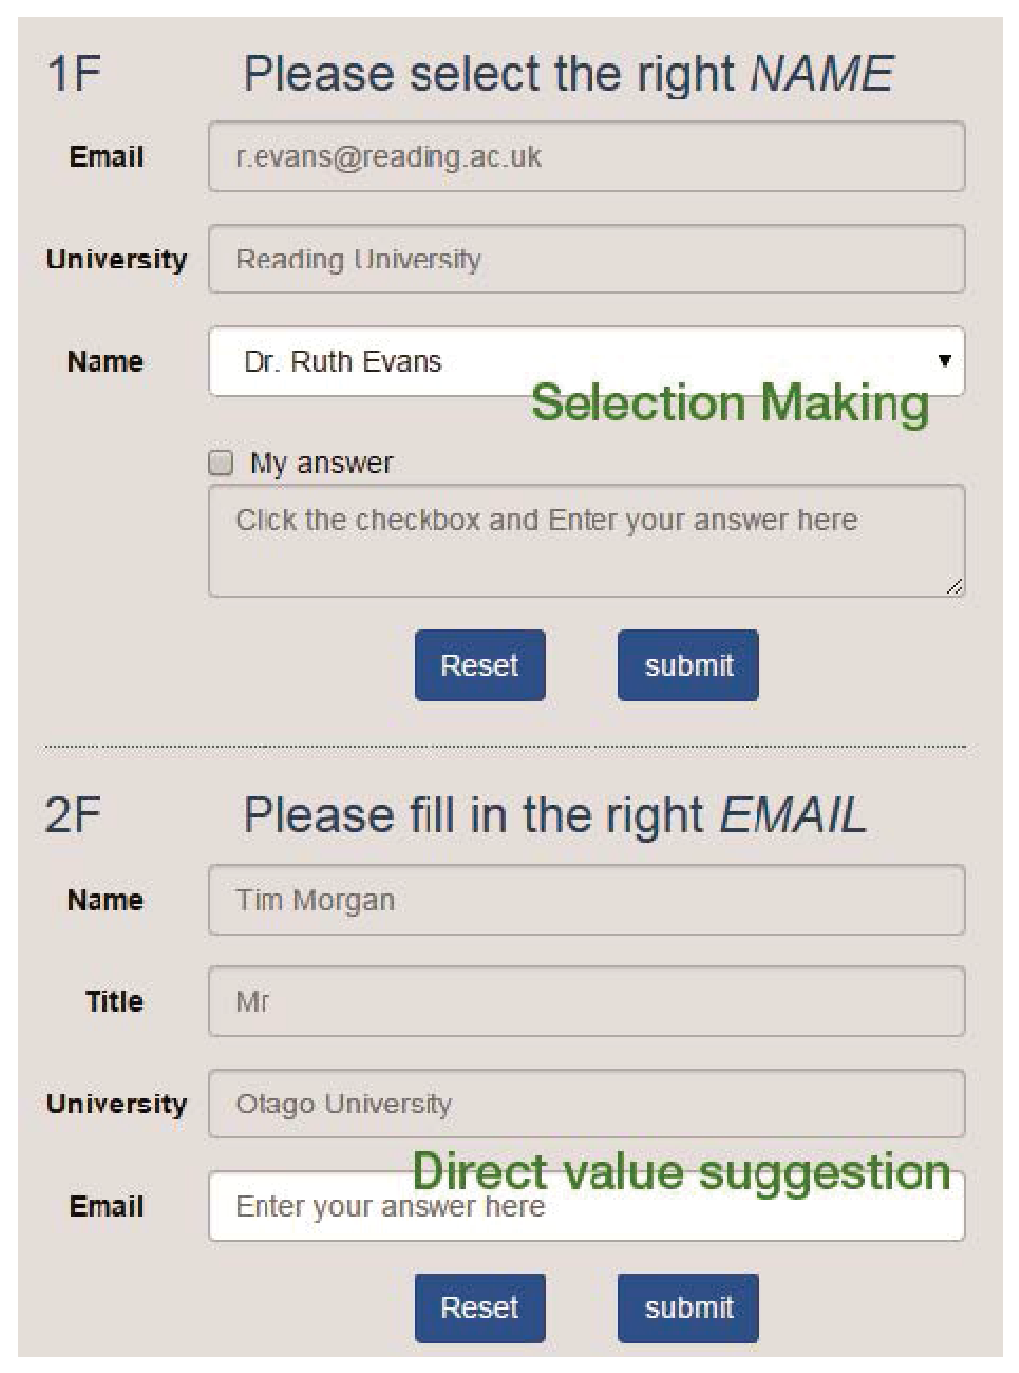
\includegraphics[width=3cm]{images/crowd.eps}}
  \caption{\small Two Types of Crowdsoucing Tasks}
  \label{fig:crowdsource}
\end{figure}


{\color{red}Firstly, the inferring step fills all inferred missing values to the maximum extent. Secondly, the subsequent retrieval step retrieves a selected set of missing values so that a set of unfilled missing values can be inferred at the next inferring step. We keep on repeating the two steps until there is no more missing values can be imputed.}
%
However, some missing values are only inferable when certain blanks are filled with specific imputed values, which can not be predicted a prior. So the selection of values for retrieving will have an impact on the succeeding inferring and retrieving step.

To achieve the optimal scheduling scheme {\color{red}that can fill all missing values at the minimum web consultation cost}, the basic rule is to retrieve only two kinds of values: 1) those cannot be inferred even all the other missing values are imputed (un-inferable), and 2) those form an {\em inference deadlock} with some other missing values, where an inference deadlock refers to a group of missing values, in which each value in the group is possible to be inferred only when some other values in the group are imputed firstly.
%
In our implementation, we build an inference dependency graph when it comes to the retrieving step, and then introduce a scheduling algorithm to identify the minimum set of missing values for retrieving. More details about this have to be omitted due to space limitation and can instead be found in~\cite{li2015trip}.

\vspace{-10pt}
\subsection{Crowdsourced Interventions}
%In principle, it is highly adaptable to specify the contents for crowdsourcing for the sake of privacy issue such as salary and age.
%
A crowdsourcing module is incorporated to have the crowds help make decisions when we have multiple qualified answers or directly input an answer for a particular missing value.
%
The basic workflow can be described as follows: when multiple answers with reasonable confidence are gotten, the one(s) with the highest confidence will be temporarily adopted in an intermediate table, and a crowdsourcing task will be generated with all these answers.
%
Crowd workers who login the system will be presented with a user-friendly interface for each particular task containing: 1) a {\em selection box} for users to select from a list of limited options; 2) a pure {\em input box} for inputting other answer, and 3) some {\em extra information} about the missing value in the task, such as the existing attribute values in the same tuple.
%
Two types of tasks are listed in Fig.~\ref{fig:crowdsource}.


\begin{figure*}[t]
  % Requires \usepackage{graphicx}
  \setlength{\abovecaptionskip}{0pt}
  \centerline{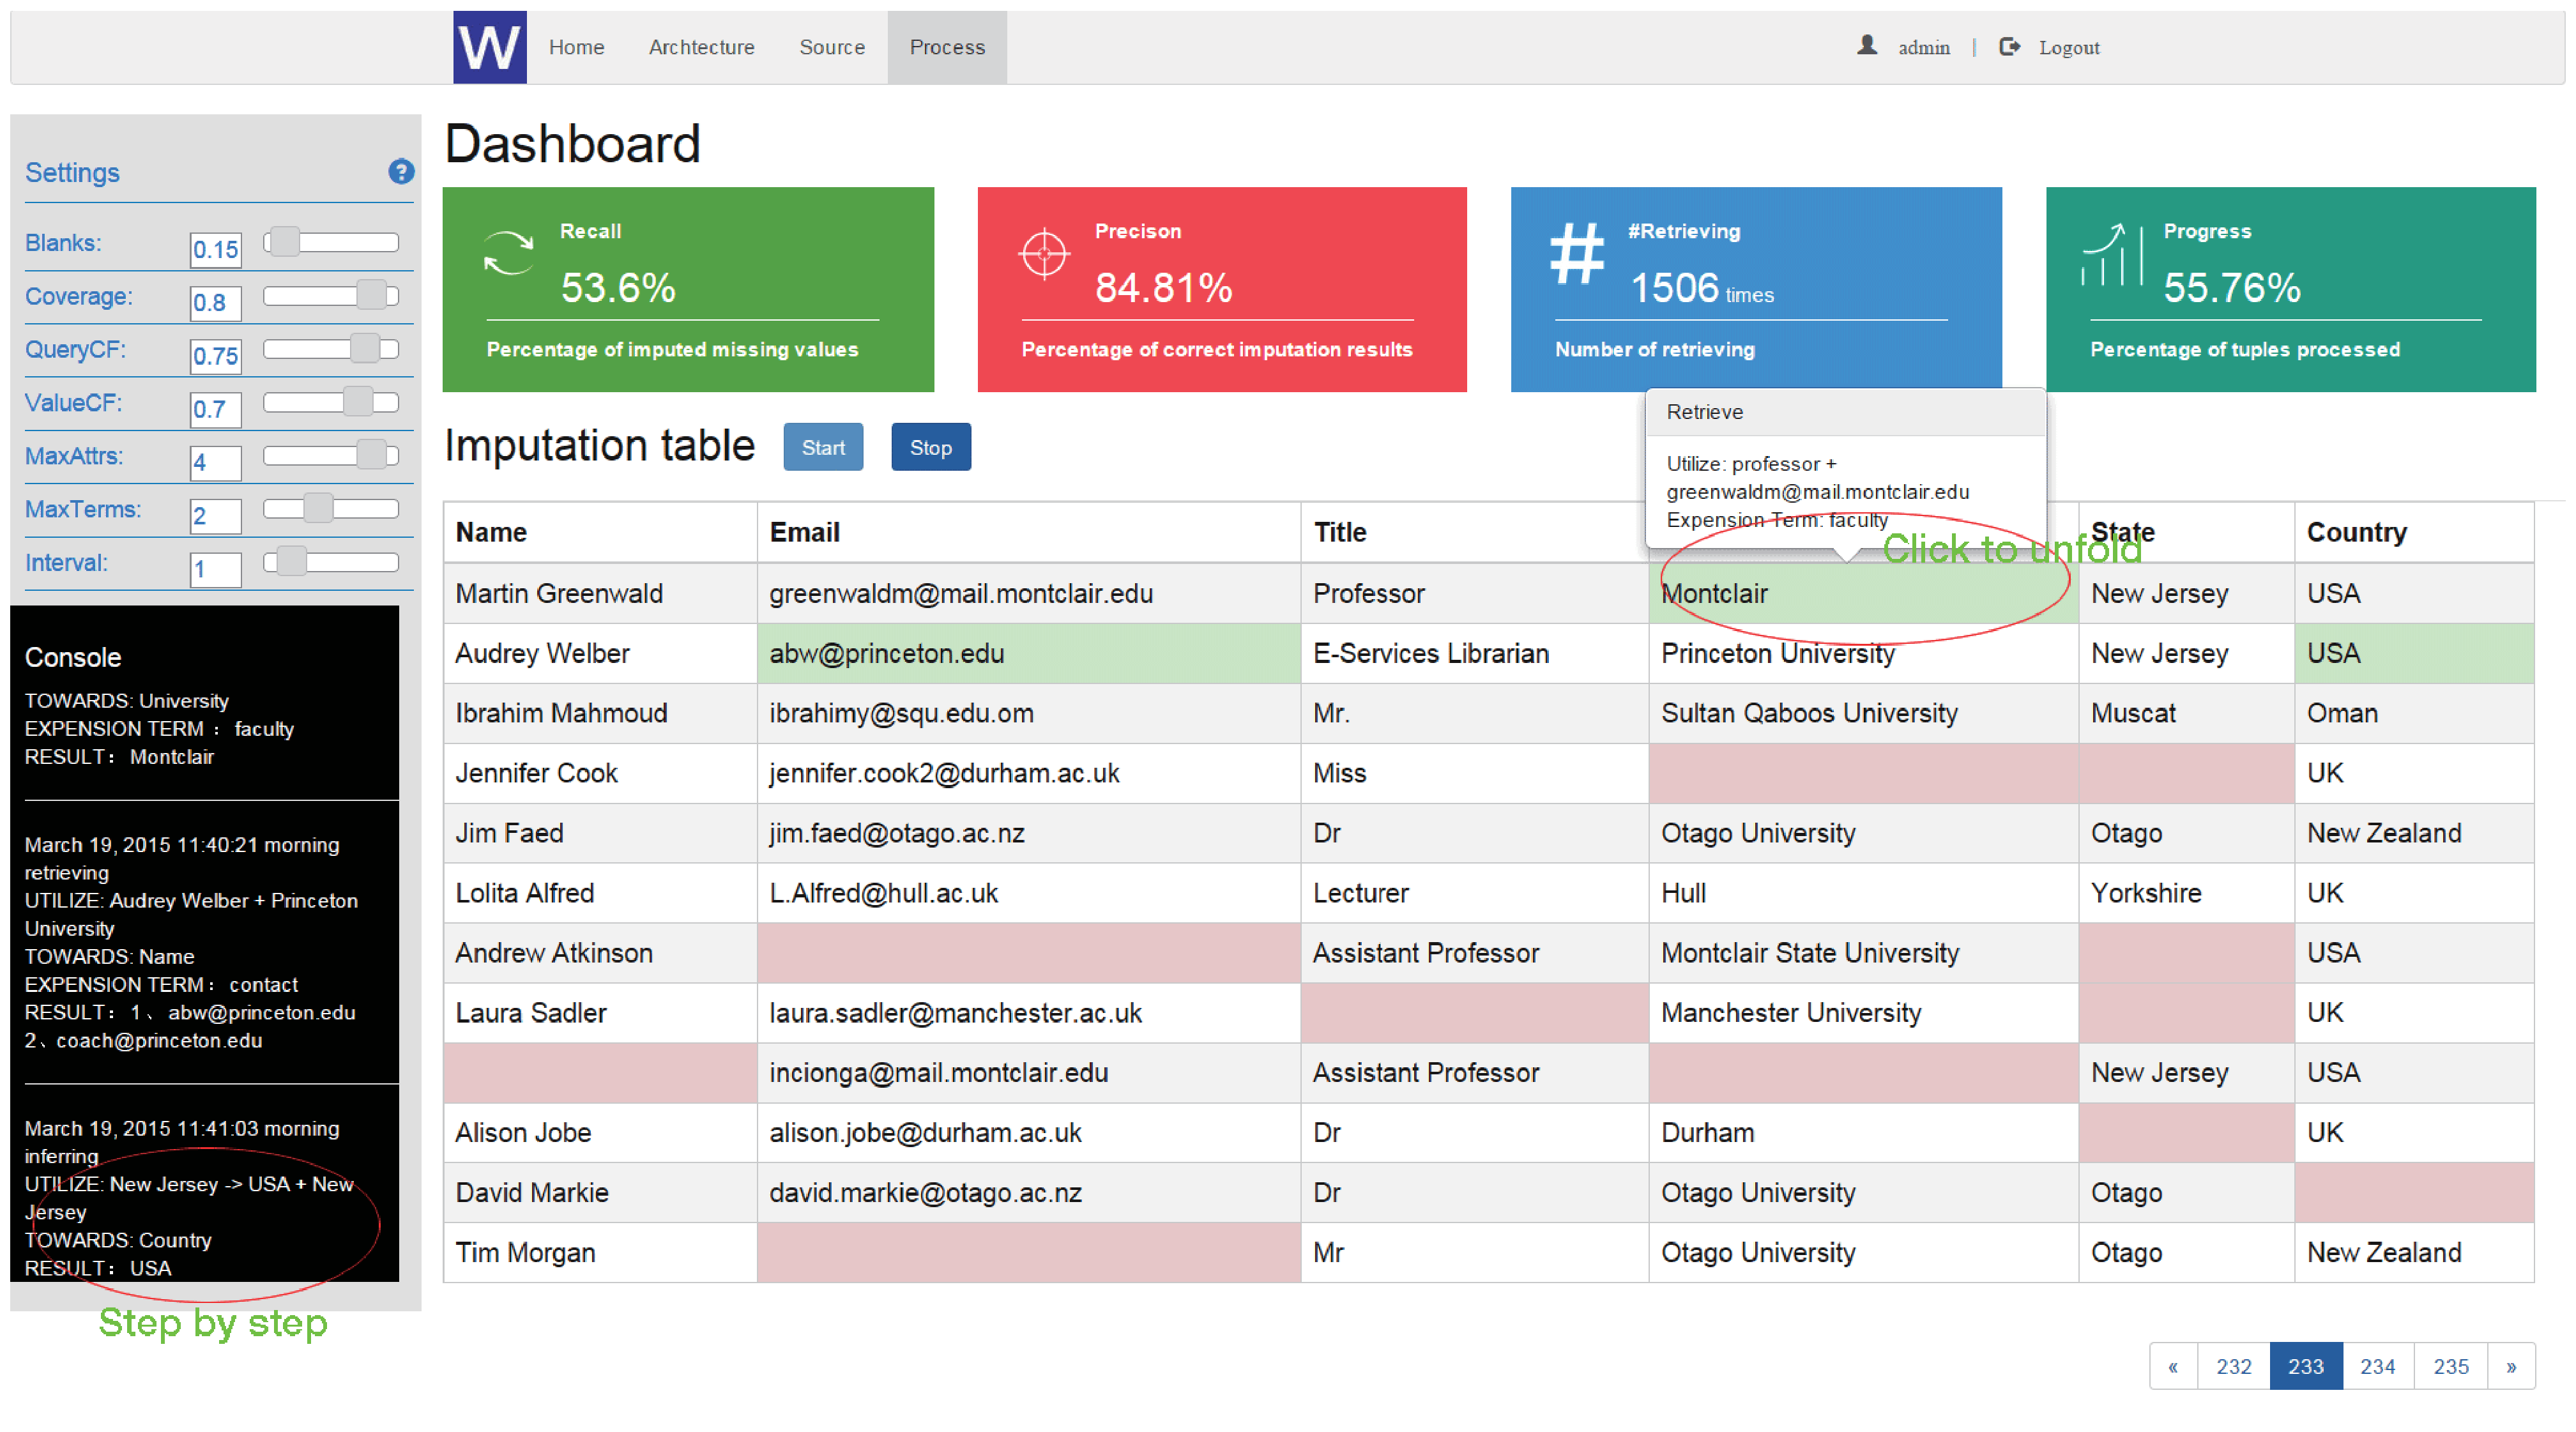
\includegraphics[width=11cm]{images/process_.eps}}
  \caption{ \small Demonstration of Imputing Process of WebPut}
  \label{fig:process}
\end{figure*}

%{\color{red} In order to obtain high quality results, we have designed a rule that workers's earnings is determined by their overall contribution to the missing values.}
%
WebPut incorporates mechanisms for checking the correctness of the input values such as the data type and format. In addition, in the presence of malicious workers, we deliberately add some evaluation questions in the list of questionnaire, answers of which are already known, and the credibility of each crowd worker is assessed by how well the input answers fit the right answers.
%
WebPut is designed to solve tasks in parallel, thus multiple workers can asynchronously fulfill the imputing tasks. When there are conflicts between the input answers from different workers, a voting mechanism is employed to consider both the popularity of an answer and the credibility of relevant crowd workers. Workers whose credibility is higher than others have priority to fulfill tasks.
%{\color{red}Workers will be rated by this voting mechanism and workers with high scores will be given priority in data imputation tasks.}

\vspace{-10pt}
\section{DEMONSTRATION}

We plan an end-to-end demonstration, which visualizes the whole workflow from setting up the system's parameters all the way to exhibiting the final imputation results and some detailed reports on how each value is imputed and the overall statistical reports.
%
The {\em Personal Contact Information} data set we employ for demonstration is a 7-attributes (Name, Email, Title, University, Country, State, Postcode), 50k-tuples relational table, collected from 100+ universities worldwide.

\noindent{\bf 1) Web-based Operations Demonstration:}
We show the fresh users with some background knowledge of data imputation and then describe in a top-down style how WebPut works in fetching expected web document that hopefully contains the desired attribute values and extracting the desired candidate values from the web pages.


\noindent{\bf 2) Step-by-Step Interactive Imputation:}
WebPut can exhibit the process of interactive inferring and retrieving step by step as shown in Fig.~\ref{fig:process}. By default, we set the imputation interval to 1s for visualization purpose. And users can change the time slots by simply dragging on the interval bar and the speed of imputation will change accordingly. Likewise, all the thresholds can be customized during the demonstration.


\noindent{\bf 3) Unfold Imputation Process:} In addition to displaying imputed results, WebPut keeps track of how each imputation value comes into being. As a result, if users are curious about how a specific missing value is imputed, they can double click on the data item and imputation information related to that data will popup. %These provenance information is of great significance to researches, for whom the source where these imputed data come from matters.

\noindent{\bf 4) Live Interaction (User or Crowd Worker Input):}
This is the most interesting part. Every CIKM attendee is encouraged to participate in the demonstration either as a user or as a crowd worker. As a user, one can name a new data set for imputation or input any new person's name and email to the current data set to see if WebPut can get all the rest contact information for the person. As a crowd worker, one can experience how a worker works in the system.
% as crowdsourcing workers. During the demonstration, users can simply login our system and help to improve imputed result. %\Change{\sout{The contributions of crowd workers can be visually exhibited on the dashboard.}}
%
Also, we will make our system online after the conference.

%\vspace{-3pt}
\bibliographystyle{ACM-Reference-Format}
\bibliography{References}

\end{document}
